\documentclass{beamer} 

\beamertemplatenavigationsymbolsempty

\usetheme{Madrid}

\usepackage{pdfpages}
\usepackage[utf8x]{inputenc}
\usepackage{url}
\usepackage{graphicx}
\usepackage{adjustbox}
\usepackage{ragged2e}
\usepackage{verbatim}
\usepackage{textpos}
\usepackage{lmodern,textcomp}
 \setbeamertemplate{enumerate items}[default]
 \setbeamertemplate{itemize items}[circle]
 \setbeamertemplate{frametitle continuation}{}
\setbeamertemplate{section in toc}[circle]
\setbeamertemplate{subsection in toc}[circle]

\usepackage{soul}
\usepackage{hyperref}

%%%%%%%%%%%%%%%Color%%%%%%%%%%%%%%%
\definecolor{KIPlum}{HTML}{880052}
\definecolor{box}{RGB}{250, 117, 144}
\usecolortheme[named=KIPlum]{structure}

%%%%%%%%%%%%%%%Title page%%%%%%%%%%%%%%%

\title[Thesis Journey at MPH]{Thesis Journey at MPH, Epidemiology }
\date{31 August 2020}
\author[Enoch Yi-Tung Chen]{Enoch Yi-Tung Chen\textsuperscript{1,2}}
\institute[]{
\textsuperscript{1}Master's Program in Public Health Sciences Epidemiology (2018-2020) \\
\textsuperscript{2}Research Assistant at Department of Medical Epidemiology and Biostatistics 
\\ Karolinska Institutet}

%%%%%%%%%%%%%%\begin{document}%%%%%%%%%%%%%%%%

\begin{document}

\begin{frame}
\maketitle 
\end{frame}

\begin{frame}

\frametitle{Outline}
\hfill
\parbox[t]{.95\textwidth}{
  \begin{minipage}
  {\textwidth}
  \tableofcontents
  \end{minipage}
}
     
\end{frame}

%%%%%%%%%%%%%%%%%%%%%%%%%%%%%%%%%%%%%%%%%%%%%%%

\section{Story behind my thesis}

\begin{frame}{Story behind my thesis}
\begin{itemize}
	\item<1-> (Jun 2019) Finished my first year at KI 
	\item<2-> Interested in health economics
	\item<3-> Got in touch with a former professor of mine
	\item<4>  (Jul \& Aug 2019) Did a summer internship 	back to Taiwan
\end{itemize}
\end{frame}

\begin{frame}{Story behind my thesis}
\center
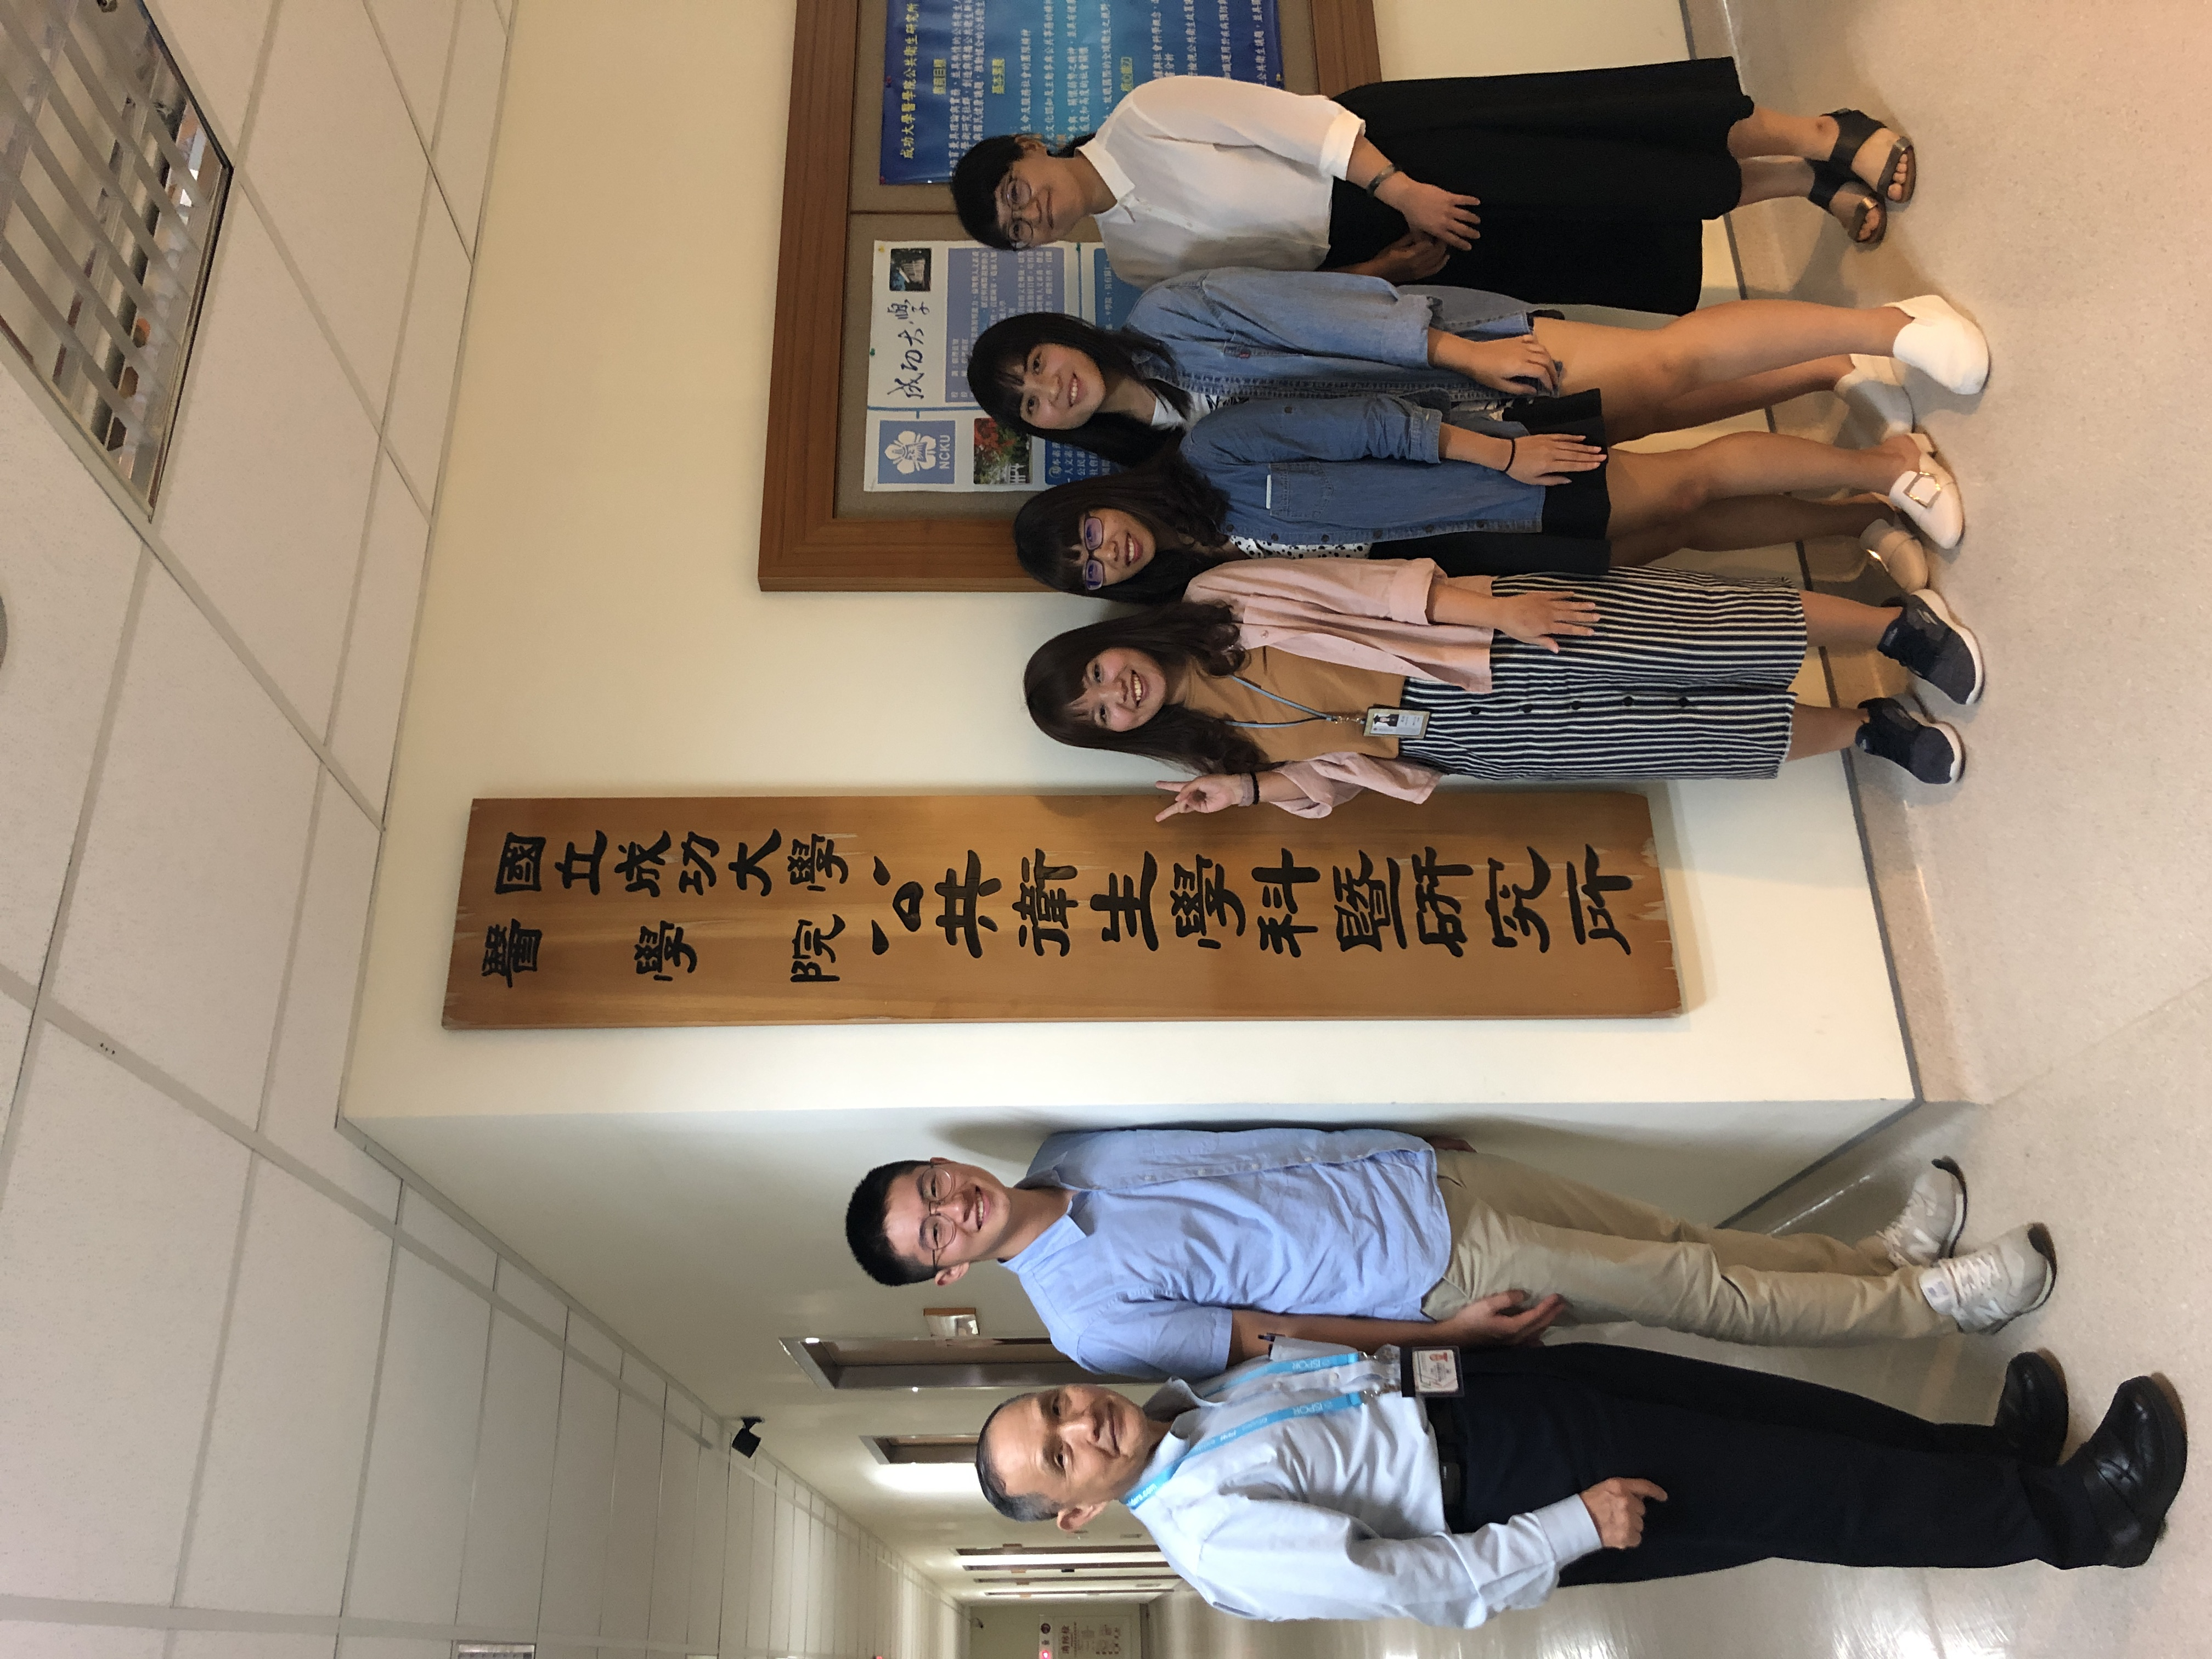
\includegraphics[width=6cm, height=8cm]{image/IMG_4994}
\end{frame}

\begin{frame}{Story behind my thesis}

\begin{itemize}
\item[]<1->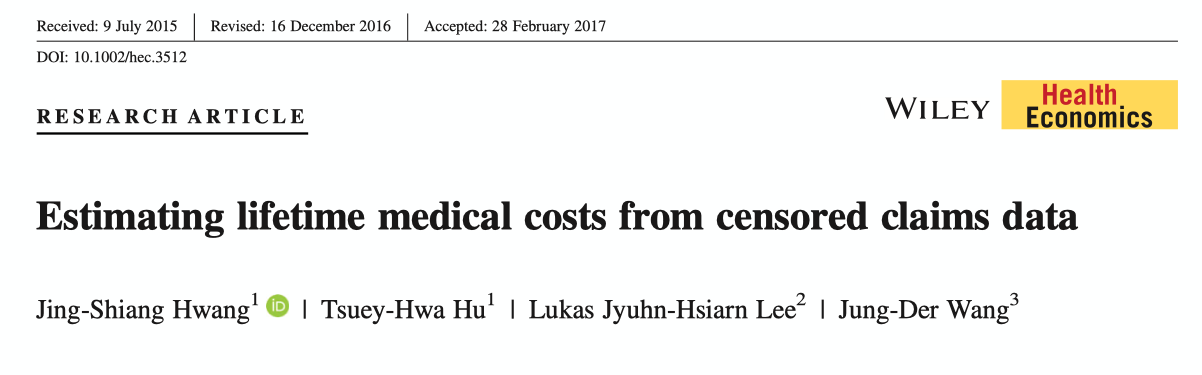
\includegraphics[width=11cm,height=3.5cm]{image/Hwang_2017}
\item[]<2->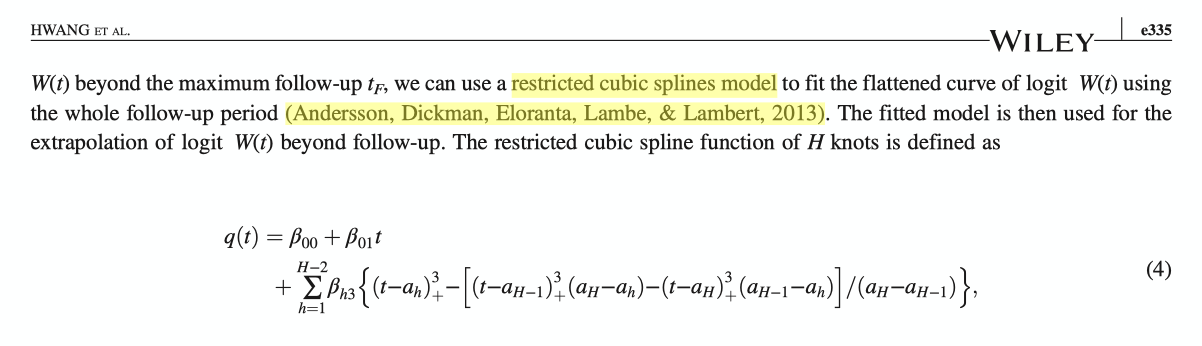
\includegraphics[width=11cm,height=3cm]{image/Hwang_2017_rcs}
\end{itemize}

\end{frame}




\begin{frame}{Story behind my thesis}

\includegraphics[width=10cm,height=5cm]{image/Andersson_2013}
\end{frame}


\begin{frame}{Story behind my thesis}
\begin{itemize}
	\item<1->  Asked to do my master's thesis with the team at MEB, KI
	\item<2->  (Sep 2019) Accepted as a thesis student at the Biostat group at MEB 
	\item<3->  (Sep-Dec 2019) Project plan period (still taking full-time courses) 
	\item<4>   (Jan-Jun 2020) Thesis period \st{Covid period is not yet done. :(}
\end{itemize}
\end{frame}

%%%%%%%%%%%%%%%%%%%%%%%%%%%%%%%%%%%%%%%%%%%%%%%

\section{About my thesis}
\begin{frame}{About my thesis}

\begin{itemize}
	\item<1-> Title: Extrapolating cancer patient survival: a comparison of the flexible parametric model and the rolling-over algorithm	
	
	\item[]<2->\begin{figure}
	\begin{center}
	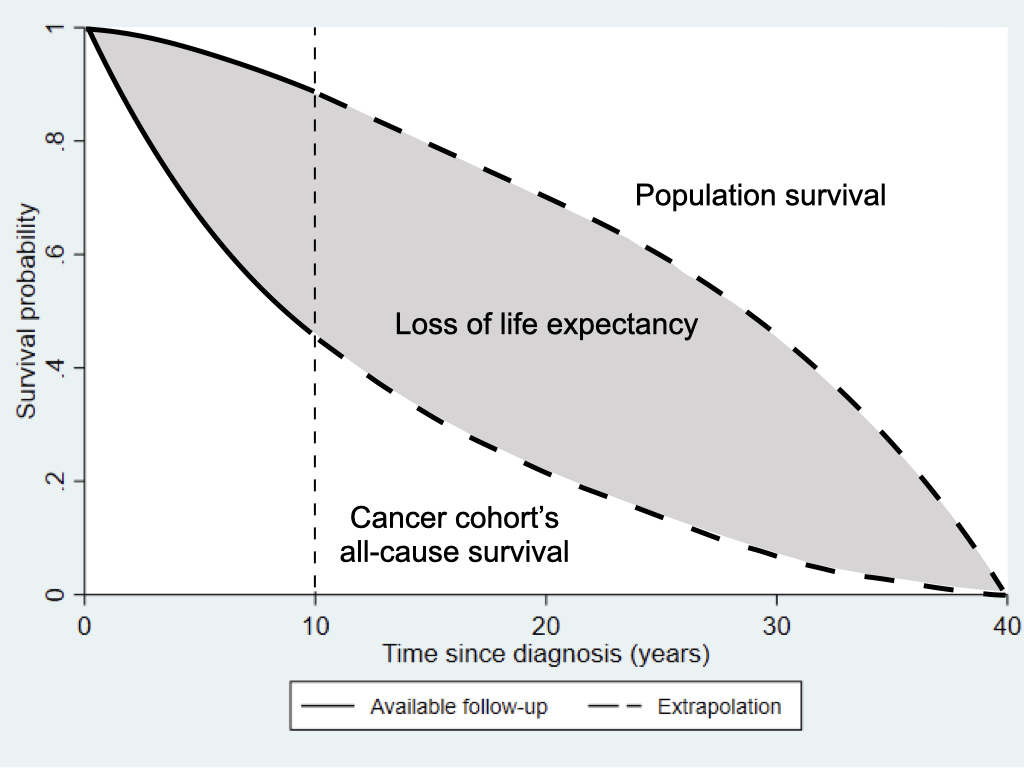
\includegraphics[scale=0.18]{image/LLE_edit}
	\caption{\centering Graphical illustration of loss of life expectancy}
	\end{center}
\end{figure}
\end{itemize}
\end{frame}

%%%%%%%%%%%%%%%%%%%%%%%%%%%%%%%%%%%%%%%%%%%%%%%
\begin{frame}[allowframebreaks]{About my thesis}

Both these two methods adopt restricted cubic splines, shown below
\begin{equation}
s(x)=\sum_{j=0}^{n} \beta_{0 j} x^{j}+\sum_{i=1}^{K} \sum_{j=0}^{N} \beta_{i j}\left(x-k_{i}\right)_{+}^{j},
\end{equation}

Cubic splines, where $N$=3, are the most common use of spline function,  shown as 

\begin{equation}
s(x)=\sum_{j=0}^{3} \beta_{0 j} x^{j}+\sum_{i=1}^{K} \beta_{i 3}\left(x-k_{i}\right)_{+}^{3}
\end{equation}

If a cubic spline function is forced to be linear before the first knot and after the last knot, then we obtain restricted cubic spline function, which is written as 
\begin{equation}
s\left(x ; \gamma_{0}\right)=\gamma_{00}+\gamma_{01} v_{1}(x)+\gamma_{02} v_{2}(x)+\ldots+\gamma_{0 K-1} v_{K-1}(x),
\end{equation}

\framebreak
\center
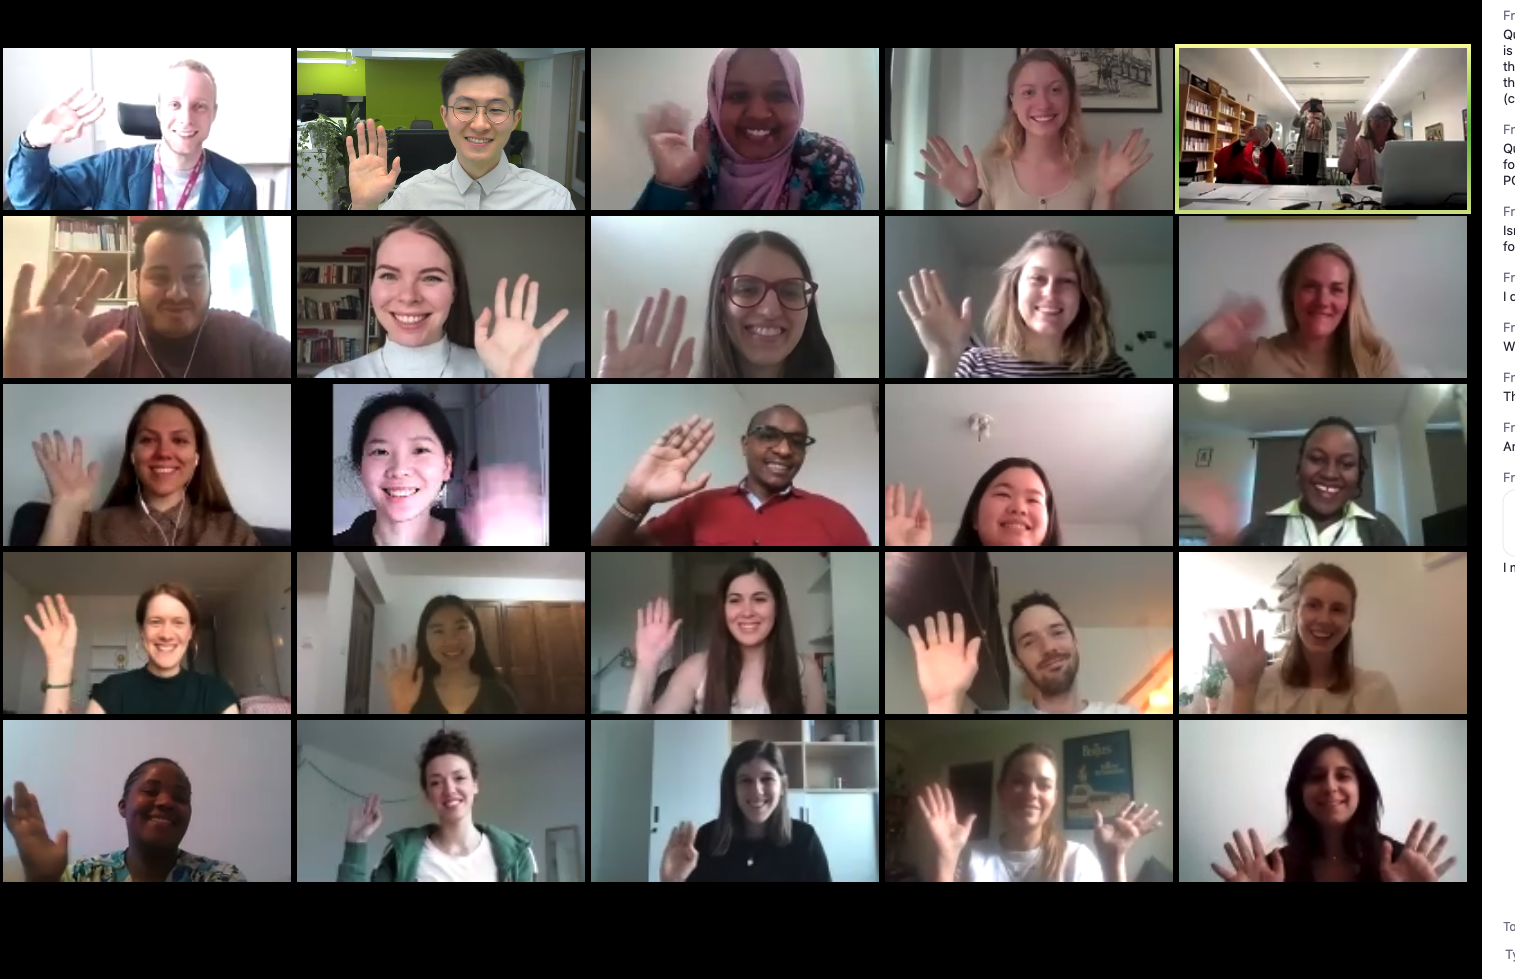
\includegraphics[width=10cm,height=7cm]{image/defensephoto}

\framebreak
\center
\includegraphics[width=10cm,height=7cm]{image/DSCF5044}

\end{frame}

%%%%%%%%%%%%%%%%%%%%%%%%%%%%%%%%%%%%%%%%%%%%%%%
\begin{frame}{Learning during my thesis period?}

\begin{itemize}
	\item <1->  Speed is important. Direction is even more important.
	\item <2-> Peer review. (Those newbies sitting beside you are way too valuable.)
	\item <3-> We are at the place with treasure	.
\end{itemize}
\end{frame}


\begin{frame}[allowframebreaks]{Learning during my thesis period?}

\center

\includegraphics[scale=0.4]{image/Gol-D-Roger-Is-Luffy.jpg} \\
Gol.D.Roger said to Monkey D. Luffy, \\"My fortune is yours for the taking, \\
but you'll have to find it first.\\ I left everything I own in One Piece." \\

\tiny (Figure: https://kledikun.blogspot.com/2017/12/goldroger-or-monkeydluffy.html)


\end{frame}

%%%%%%%%%%%%%%%%%%%%%%%%%%%%%%%%%%%%%%%%%%%%%%%
\section{What were our thesis topics?}
\begin{frame}{What were our thesis topics?}
		\begin{figure}
		\center
		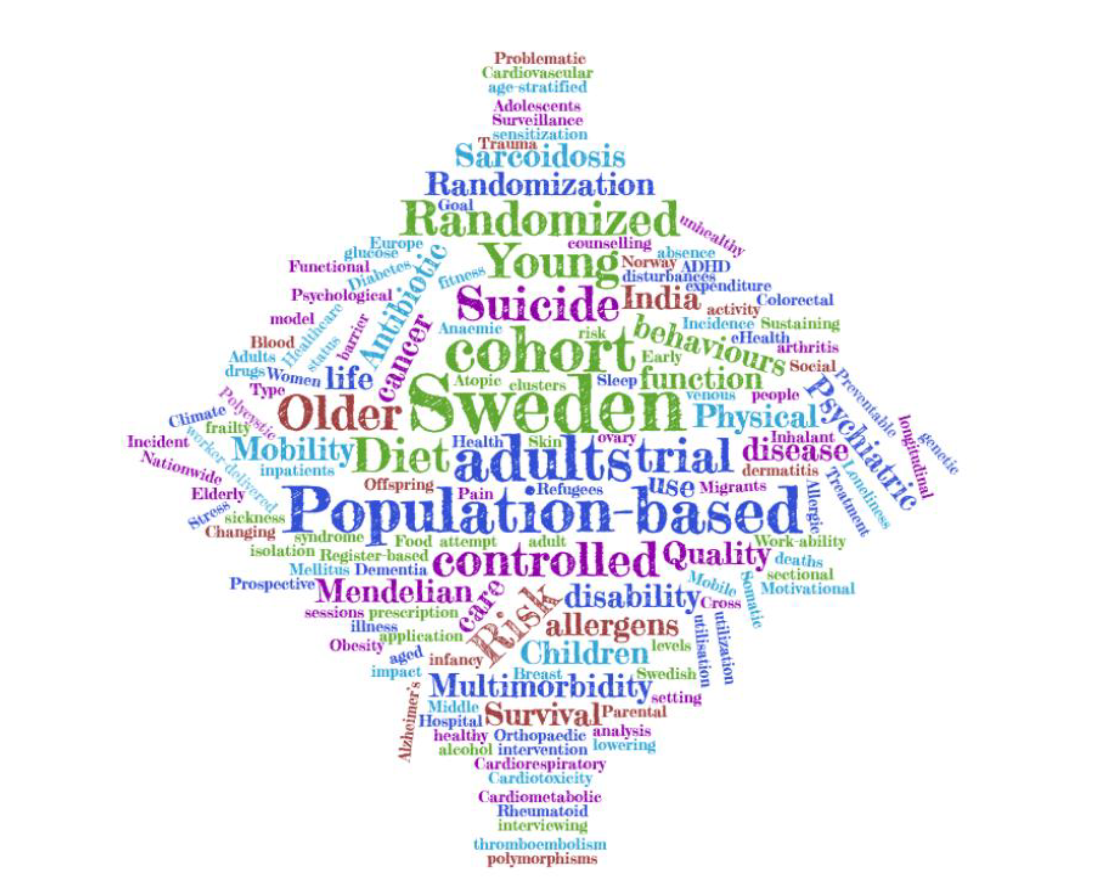
\includegraphics[scale=0.4]{image/thesistopics}
		\caption{\small Thesis topics of MPH class of 2020. Figure credit: Newsletter to master students, Department of Global Public Health, July 2020}
		\end{figure}

		
\end{frame}

%%%%%%%%%%%%%%%%%%%%%%%%%%%%%%%%%%%%%%%%%%%%%%%
\section{How did we find thesis topics?}
\begin{frame}{How did we find thesis topics?}
\begin{itemize}
	\item <1-> Thesis project proposals (sent out by Program director)
	\item <2-> Summer internship $\rightarrow$ thesis student 
	\item <3-> Fieldwork
	\item <4-> Original connection $\rightarrow$ KI connection
	\item <5>  Erasmus
\end{itemize}
	
\end{frame}

%%%%%%%%%%%%%%%%%%%%%%%%%%%%%%%%%%%%%%%%%%%%%%%

\section{Feasibility vs. Interest}
\begin{frame}{Feasibility vs. Interest}
	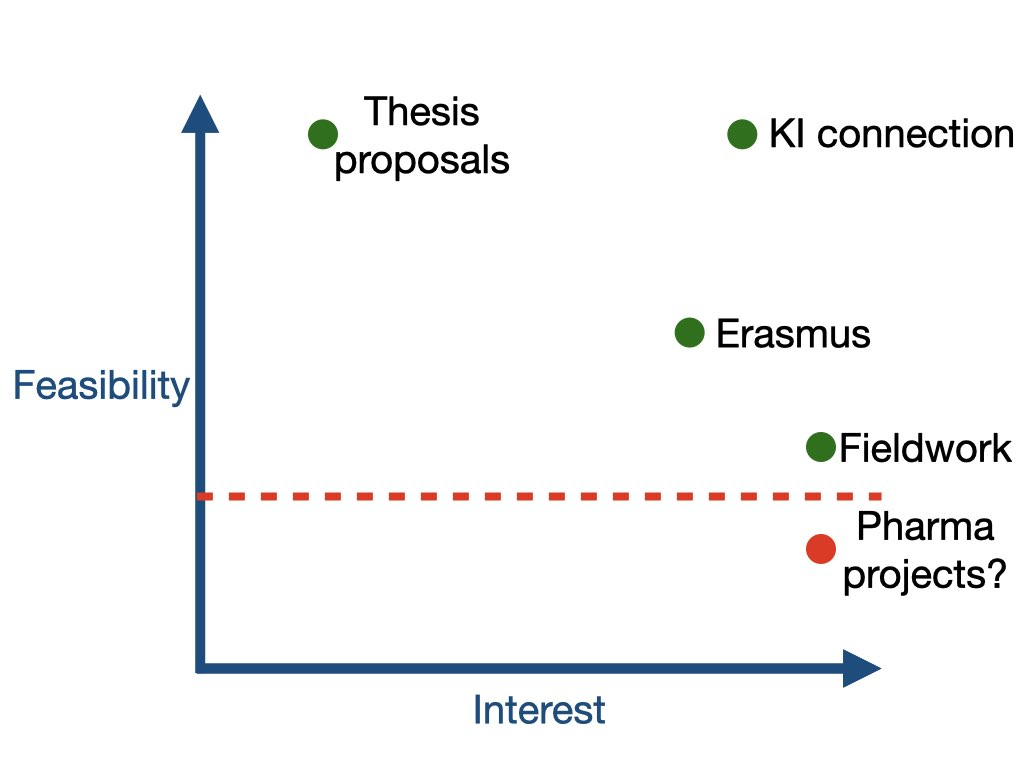
\includegraphics[scale=0.3]{image/feasibility_interest/feasibility_interest.001.jpeg}
\end{frame}

\begin{frame}{Feasibility vs. Interest}
	\begin{itemize}
	\item Feasibility: 
	      \begin{itemize}
	      \item<1-> Need to a PASS to get the diploma
	      \item<2-> Minimum	 thesis criteria (25 pages, 4 months, defense, no plagiarism)
	      \item<3-> \st{PhD thesis}, \st{Change the entire world}
	      \item<4-> \st{Nobel prize (though you are at KI)}
	      \end{itemize}
	\item<1->  Interest:
		 \begin{itemize}
		 \item<5-> You can feel happy when doing your thesis.

		 \end{itemize}
		\end{itemize}
\end{frame}

%%%%%%%%%%%%%%%%%%%%%%%%%%%%%%%%%%%%%%%%%%%%%%%
\begin{frame}{You need friends}
	\center
	
\includegraphics[scale=0.3]{image/snoopy}\\
	\small{Figure: https://www.pinterest.com/pin/450289662716760457/}
\end{frame}


%%%%%%%%%%%%%%%%%%%%%%%%%%%%%%%%%%%%%%%%%%%%%%%

\begin{frame}{Contact info}

\frametitle{Contact info}
\textbf{Enoch Yi-Tung Chen}\\

enoch.yitung.chen@ki.se\\
enochytchen.com\\

Slides available at: \url{https://enochytchen.com/talk/mphthesis}

\end{frame}

\end{document}